\section{Theoretischer Hintergrund}
Um den theoretischen Hintergrund dieses Versuchs verstehen zu können, wird im folgenden auf den Leistungsbeiwert $c_{p}$, den Momentenbeiwert $c_{m}$ und den Schubbeiwert $c_{s}$ eingegangen. Abschließend wird noch auf die Windgeschwindigkeiten und deren Verzögerung eingegangen.
\subsection{Der Leistungsbeiwert \texorpdfstring{$c_P$}{}}
Der Leistungsbeiwert $c_{p}$ ist wie folgt definiert.
\begin{equation}
  c_{p}= \frac{P_{WEA}}{P_{Wind}}
    \label{eq:230609_1531-Leistungsbeiwert_cp}
\end{equation}
\begin{equation}
  c_{p}= \frac{M \cdot 2 \cdot \pi \cdot n_{Rotor}}{\frac{\rho_{Luft}}{2}\cdot \pi \cdot \frac{d^2_{Rotor}}{4} \cdot v^3_{Wind} }
    \label{eq:230609_1532-Leistungsbeiwert_cp}
\end{equation}
Wie in \autoref{eq:230609_1531-Leistungsbeiwert_cp} zu sehen bildet sich $c_P$ aus dem Quotienten der Mechanischen- und der Windleistung. 
In \autoref{eq:230609_1532-Leistungsbeiwert_cp} ist dabei zu sehen wie $c_P$ von Anlagenspezifischen Eigenschaften beeinflusst wird.
Typischerweise wird der Leistungsbeiwert $c_P$ dabei über die Schnelllaufzahl $\lambda$ aufgetragen. Dabei bildet die Schnelllaufzahl das Verhältnis der Umfangsgeschwindigkeit an der Blattspitze $u_{tip}$ zur ungestörten Windgeschwindigkeit ab wie in Formel \ref{eq:Schnelllaufzahl} zu sehen.
\begin{equation}
\lambda=\frac{u_{tip}}{u_{Wind}}=\frac{\pi \cdot n_{Rotot \cdot d_{Rotor}}}{v_{Wind}}
    \label{eq:Schnelllaufzahl}
\end{equation}

\begin{figure}[h!]
    \centering
    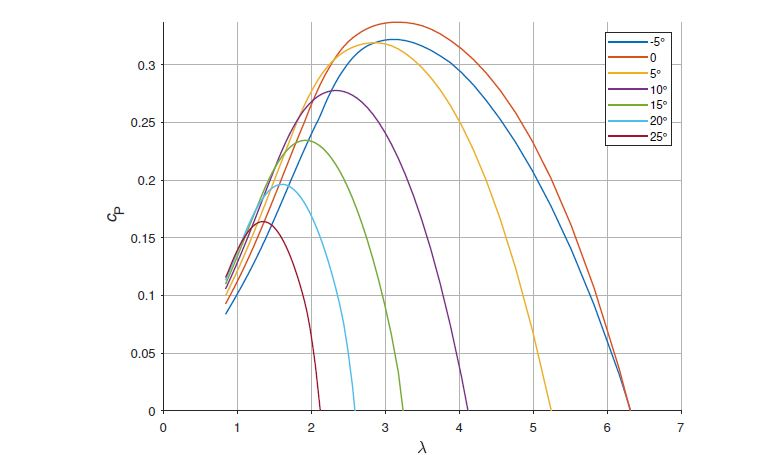
\includegraphics[width=0.5\textwidth]{Abbildungen/cpzulambda.jpg}
    \caption{Berechnete Leistungsbeiwerte $c_P$ des Rotors der Labor-Windkraftanlage in Abhängigkeit der Schnelllaufzahl $\lambda$ für unterschiedliche Blatt (Pitch-)Winkel.\cite{Anleitung}}
    \label{fig:cpzulambda}
\end{figure}

\subsection{Der Momentenbeiwert \texorpdfstring{$c_M$}{}}
Der Momentenbeiwert beschreibt das Betriebsverhalten des Rotors bezüglich der Drehmomentabgabe, mit dessen Hilfe sich eine Aussage über das Anlaufverhalten aus dem Stillstand machen lässt. Dabei ergibt er sich aus dem Verhältnis des abgegebenen Drehmoments zum Luftkraftmoment, dass auf die Rotorfläche wirkt.
\begin{equation}
  c_{M}= \frac{M}{ \frac{\rho_{Luft}}{2}\cdot \pi \cdot \frac{d^3_{Rotor}}{8} \cdot v^2_{Wind} }
    \label{eq:Momentenbeiwert_cm}
\end{equation}
Des Weiteren gilt der Zusammenhang:
\begin{equation}
  c_{M}= c_{p} \cdot \lambda
    \label{eq:Momentenbeiwert_cm2}
\end{equation}
Bei Schnellläufern ist der Momentenbeiwert beim Anlaufen sehr gering. Dies ist Bauartspezifisch bei Schnellläufern und in Abbildung \ref{fig:cmzulambda} zu sehen. 
\begin{figure}[h!]
    \centering
    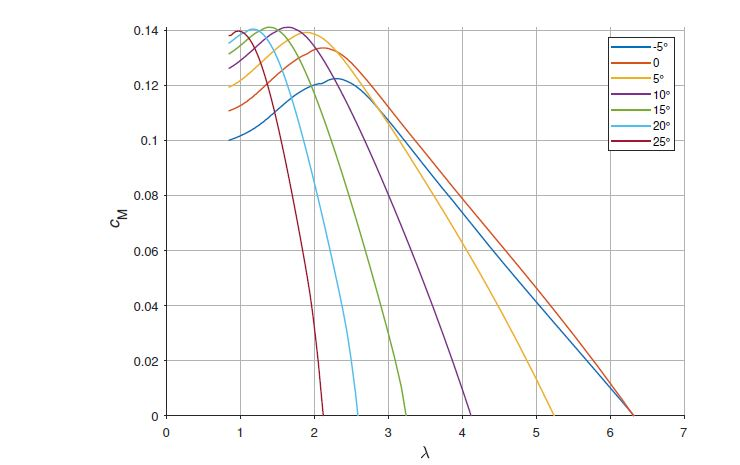
\includegraphics[width=0.5\textwidth]{Abbildungen/cm.jpg}
    \caption{Berechnete Momentenbeiwert $c_{M}$ des Rotors der Labor-Windkraftanlage in Abhängigkeit der Schnelllaufzahl $\lambda$ für unterschiedliche Blatt (Pitch-)Winkel. }
    \label{fig:cmzulambda}
\end{figure}
Noch quelle in die Abbildung (Skript Twele)

\subsection{Der Schubbeiwert \texorpdfstring{$c_S$}{}}
Der Schubbeiwert $c_{s}$ ist sehr wichtig um die Windkraftanlage Struktur-mechanisch zu dimensionieren.  Dabei ergibt der Schubbeiwert aus der dynamischen Staukraft auf die Rotorfläche.
\begin{equation}
  c_{s}= \frac{F_{S}}{\frac{\rho_{Luft}}{2}\cdot \pi \cdot \frac{d^2_{Rotor}}{4} \cdot v^2_{Wind}}
    \label{eq:Schubbeiwert_cs}
\end{equation}
Der Schubbeiwert hat sein Minimum im Stillstand und sein Maximum im Leerlauf. Hier entspricht der Widerstandsbeiwert etwa dem einer Scheibe. Höhere Schubbeiwerte bedeuten, dass sie die Windkraftanlage im Propelerbetrieb befindet.
\begin{figure}[!ht]
    \centering
    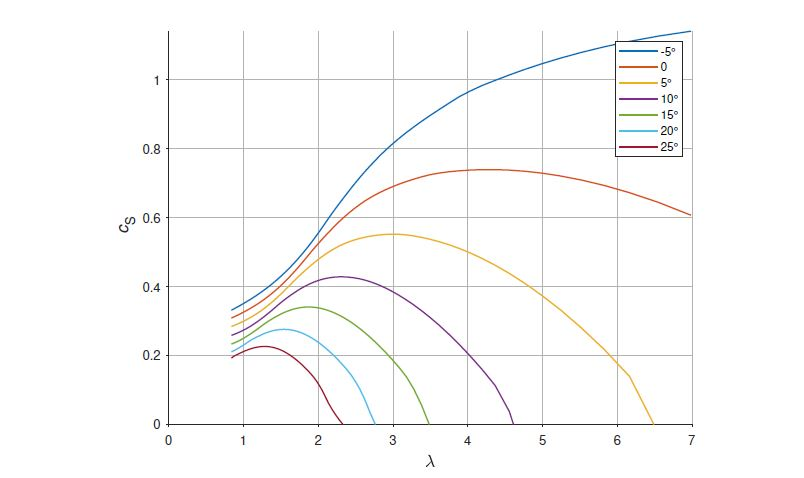
\includegraphics[width=0.5\textwidth]{Abbildungen/cszulambda.jpg}
    \caption{Berechneter Schubbeiwert $c_{s}$ des Rotors der Labor-Windkraftanlage in Abhängigkeit der Schnelllaufzahl $\lambda$ für unterschiedliche Blatt (Pitch-)Winkel.}
    \label{fig:cszulambda}
\end{figure}
Wieder Quelle rein!!!
\subsection{Verzögerung der Windgeschwindigkeit}
Wie von Betz beschrieben liegt der optimale Arbeitspunkt einer Windkraftanlage bei einem Verhältnis von $v_{1} \cdot \frac{1}{3}=v_{3}$  \ref{fig:Betz2905}. Dabei ist in Abbildung \ref{fig:Glauert} noch die Erweiterung von Glauert zu sehen, der die maximale Verblockung der Stromröhre im Leerlauf als Grenzfall berücksichtigt.
\begin{figure}[h!]
    \centering
    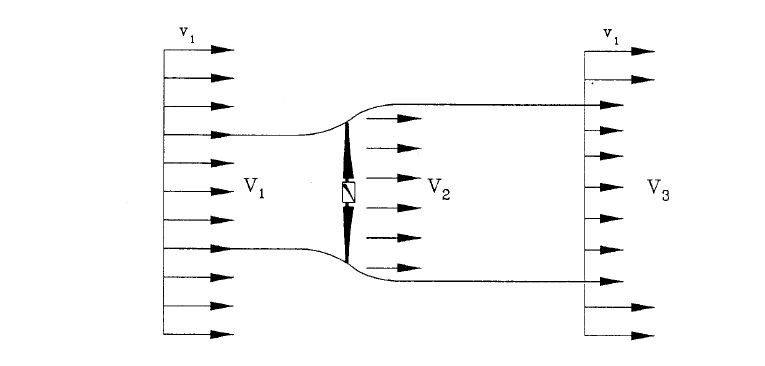
\includegraphics[width=0.5\textwidth]{Abbildungen/Betz.jpg}
    \caption{Verzögerung in der geschlossenen Stromröhre nach Betz $v_{1} \cdot \frac{1}{3}=v_{3}$ und  $v_{1} \cdot \frac{2}{3}=v_{2} $}
    \label{fig:Betz2905}
\end{figure}
\begin{figure}[h!]
    \centering
    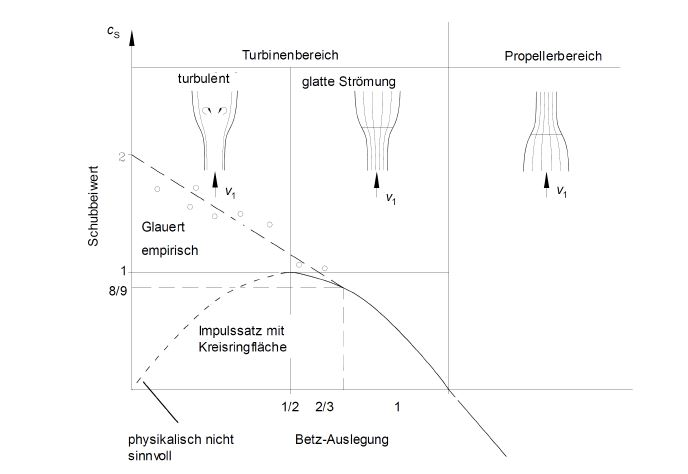
\includegraphics[width=0.5\textwidth]{Abbildungen/Glauert.jpg}
    \caption{Verzögerung in der geschlossenen Stromröhre nach Betz $v_{1} \cdot \frac{1}{3}=v_{3}$ und  $v_{1} \cdot \frac{2}{3}=v_{2} $}
    \label{fig:Glauert}
\end{figure}
